\documentclass{article}
\usepackage[utf8]{inputenc}
\usepackage[free-standing-units=true]{siunitx}
\usepackage{gensymb}
\usepackage{amsmath, amssymb}
\usepackage[T1]{fontenc}
\usepackage{url}
\usepackage{graphicx, caption, subcaption}
\usepackage{minitoc}
\usepackage[font={small,it}]{caption}
\usepackage{float}
\usepackage{multirow}
\usepackage{geometry}
\usepackage{xcolor} % to access the named colour LightGray
\definecolor{LightGray}{gray}{0.9}
\definecolor{grey}{rgb}{0.9,0.9,0.9} % Colour of the box surrounding the title
\definecolor{mygreen}{RGB}{28,172,0} % color values Red, Green, Blue
\definecolor{mylilas}{RGB}{170,55,241}
\usepackage{minted}
\usepackage{booktabs}
\setlength{\parindent}{0px} %makes paragraph indents go away
\usepackage{accents}
\usepackage{listings}
\usepackage{import}
\usepackage{xifthen}
\usepackage{pdfpages}
\usepackage{transparent}
\usepackage[version=4]{mhchem}
% Matrix notation
\newcommand{\matr}[1]{\mathbf{#1}}
\usepackage[font=small,labelfont=bf]{caption}
\usepackage[font=footnotesize]{caption}
\usepackage[british]{babel}
\usepackage{marginnote}

\DeclareSIUnit\angstrom{\text {Å}}
\newcommand\uvec[1]{\underaccent{\vec}{#1}}

\newcommand{\incfig}[1]{%
    \def\svgwidth{\columnwidth}
    \import{./resources/figures/}{#1.pdf_tex}
}

\begin{document}

\pagenumbering{roman}

\begin{titlepage} % Suppresses displaying the page number on the title page and the subsequent page counts as page 1
	
	%------------------------------------------------
	%	Grey title box
	%------------------------------------------------
	
	\colorbox{grey}{
		\parbox[t]{0.93\textwidth}{ % Outer full width box
			\parbox[t]{0.91\textwidth}{ % Inner box for inner right text margin
				\raggedleft % Right align the text
				\fontsize{50pt}{50pt}\selectfont % Title font size, the first argument is the font size and the second is the line spacing, adjust depending on title length
				\vspace{0.7cm} % Space between the start of the title and the top of the grey box
				Monte Carlo Simulation\\
				of Polymers\\
				
				\fontsize{15pt}{30pt}\selectfont
				Simulating polymers as self-avoiding random walks
				\vspace{0.7cm} % Space between the end of the title and the bottom of the grey box
			}
		}
	}
	
	\vfill % Space between the title box and author information
	
	%------------------------------------------------
	%	Author name and information
	%------------------------------------------------
	
	\parbox[t]{0.93\textwidth}{ % Box to inset this section slightly
		\raggedleft % Right align the text
		\large % Increase the font size
		{\Large Francke, A. (4713672)\\ Glorie, M. (4279492)\\ Sangers, J. (4645197)}\\[4pt] % Extra space after name
		Applied Physics - Computational Physics\\
		TU Delft\\
		05-10-2022\\[4pt]
		\hfill\rule{0.4\linewidth}{1pt}% Horizontal line, first argument width, second thickness
	}
	
\end{titlepage}

\begin{abstract}
    \chapter*{Abstract}
This report focusses on utilising scanning transmission electron microscopy in conjunction with a cutting-edge, high dynamic range direct electron detector to acquire precise and localised information on stamped moiré heterostructures. The innovative electron microscope pixelated array detector is employed to capture diffraction data from small areas of heterostructure lattices, generating a four-dimensional dataset. These datasets enable the mapping of strain, electrical, and potential fields with micrometre and nanometre level precision. A novel centre-of-mass analysis approach is developed and integrated into an existing dataset exploration framework for rapid experimentation during electron microscope data acquisition.
\end{abstract}
\newpage
\thispagestyle{empty}
\addcontentsline{toc}{section}{Table of Contents}
\tableofcontents
\clearpage
\newpage
\pagenumbering{arabic}
\section{Introduction}
% \begin{enumerate}

% \item Highlight the significance of working at the nanoscale in terms of technological advancements.

% \item Emphasise that this thesis represents a significant innovation. Mention the unique focus on the integration of 4D-STEM and EMPAD detector.

% \item Clearly state the objectives of the research. Explain the scope, which includes mapping strain, electrostatic potentials, and electric fields in van der waals heterostructures.

% \item Discuss why van der Waals heterostructures is crucial. Emphasise the potential impact on applications. 


% \item Brief outline the methodologies that will be employed, including 4D-STEM

% \item Highlight the contributions of this thesis, such as the development of code for interpreting COM.

% \item Provide an overview of how the thesis is organised, mentioning the subsequent chapters and their roles.
    
% \end{enumerate}


Two-dimensional layered materials have garnered significant attention because they exhibit exciting optical, thermal, and electronic properties that change dramatically as the material is thinned down from bulk to monolayer. The already vast amount of tunability increases even further as one starts to stack these thin two-dimensional building blocks into larger potentially twisted heterostructures. Van der Waals forces that normally hold together the layers in the bulk crystal also form the glue that holds these new heterostructures together. This relative ease in manufacturing and the potential applications in fields ranging from power electronics and solar cells to single-photon emitters and biosensors make studying these materials more than worthwhile~\cite{LI2016322, https://doi.org/10.1002/smll.202107059}.\\
Studying these fascinating materials and the dynamical interplay between the tunable physical properties such as strain, twist angle, and material combination calls for highly sophisticated and specialised characterisation techniques. Therefore, scanning transmission electron microscopy will be used in combination with a state-of-the-art, fast, and high dynamic range direct electron detector to gather highly localised information. The innovative electron microscope pixelated array detector will be used to capture the diffraction information of a small area in the heterostructure crystal lattice by scanning over the sample with a small localised electron probe in a rasterised pattern to form a four-dimensional dataset. From these four-dimensional datasets accurate strain-, electrical-, and potential-fields can be mapped with micrometre and nanometre precision, respectively. To this end a new to us centre-of-mass analysis approach will be developed and implemented in an existing dataset exploration framework used for rapid experimentation of electron microscope parameters at the time of acquisition.\\
In the report, relevant theory on electron microscopy and crystallography will be presented first in Section \ref{sec:theory} after which the fabrication of moiré heterostructures will be explained in Section \ref{sec:methods}. The EMPAD and the data sets it captures and how it will be analysed are explained in Section \ref{sec:empad}. The results stemming from the application of the new analysis techniques are explained in Section \ref{sec:results}, and finally, the conclusions and future possibilities will be discussed in Section \ref{sec:outlook}.


\newpage
\section{Transmission Electron Microscopy and Crystallography of TMDs}

\subsection{The Transmission electron microscope (TEM)}
The Transmission electron microscope (TEM) is a microscope that far exceeds the capabilities of a normal light microscope. Both types of microscope use a series of lenses to magnify the image of a specimen.
A normal light microscope can amplify an image up to about 1500$\times$ and is limited by the diffraction limit of light. Assuming an average wavelength of \SI{550}{\nm} for green light, a high-end microscope is limited to resolving features \SI{100}{\nm} apart.
This limit is insufficient for looking at atomic structures \cite{PhysRevLett.106.193905}.\\
An electron microscope circumvents this limit by using electrons, not light, to probe the specimen. Electrons when accelerated have a smaller wavelength than light thus allowing for images with resolved features as small as \SI{0.05}{\nm}. \cite{kisielowski_freitag_bischoff_van}
The TEM works by releasing electrons from an electron source and accelerating them to an energy typically expressed in kilo-electronvolt; as shown in equation \ref{eq:acc_volts}, the higher the accelerating voltage of the microscope the smaller the de Broglie wavelength of an electron, which results in a higher resolving power. Modern electron microscopes accelerate electrons up to \SI{300}{\kilo \electronvolt}

\begin{equation}
    \lambda_e = h\cdot \left[ 2 \cdot e \cdot m_e \cdot V_a \right]^{-1/2}
    \label{eq:acc_volts}
\end{equation}

\begin{figure}[h]
    \centering
    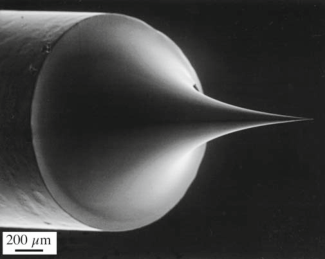
\includegraphics[keepaspectratio, width=0.5\linewidth]{resources/Figures/feg.png} 
    \caption{Pictured is the tip of a field emission gun \cite{Williams2009-ww}. The tapered tip facilitates the creation of a strongly varying potential that eases the expulsion of electrons from the material. These electrons are then accelerated along the optical axis.}
    \label{fig:feg}
\end{figure}

In a TEM the electrons are released from a field emission gun (FEG, pictured in Figure \ref{fig:feg}). 
The FEG is placed in proximity to two anodes, the first anode is positively charged to several kilovolts such that it extracts electrons from the tip of the FEG, the second anode is charged to the wanted acceleration voltage \cite{Williams2009-ww}.
FEGs are about three orders of magnitude brighter than thermionic emission electron sources \cite{field-emission}.
After being emitted the electrons pass through a monochromator that reduces the energy spread of the emitted electrons. An electron then continues along the optical axis into an illuminating system consisting of multiple electromagnetic lenses, which lenses are activated and to what extent depends on the operating mode of the electron microscope.

% \subsubsection{Bright Field}
% A bright field (BF) image of the sample is acquired by using a parallel electron beam. This beam is formed using the lens configuration shown in figure \ref{fig:tem_operating}. This parallel beam is typically several micrometers in size at magnifications up to 20k-100k$\times$.
% In normal operating mode a BF image is captured by a camera looking at a phosphorous screen or by a camera directly, this method of imaging is most analogues to a normal light microscope.
% The electron beam is focused in such a way that it illuminates the sample with a parallel beam, such a beam is also used for creating the clearest diffraction patterns.
% %A bright field image can also be formed in STEM operating mode.
% \begin{figure}[h]
%     \centering
%     \def\svgwidth{.66\linewidth}
%     \import{resources/Figures}{parallel_op_mode.pdf_tex}
%     \caption{Illumination system for parallel beam.}
%     \label{fig:tem_operating}
% \end{figure}
\subsubsection{Dark Field and Z-contrast Imaging}
For dark field and Z-contrast the electron beam is focused to a small area, this creates a higher intensity electron beam with a probe-like point as can be seen in Figure \ref{fig:stem_operating}. Since all the electrons are focused on a small area there is no contrast information that can be used to form an image. To form an image using such a beam the probe point needs to be scanned over the sample leading to the term Scanning Transmission Electron Microscopy.
Dark field images use electrons scattered away from the optical axis to form an image, to achieve this most STEMs have a series of annular dark field detectors.
These ring shaped detectors encircle the central bright field detector and can collect electrons that have been scattered at various angles. Normal dark field detectors collect electrons scattered up to an angle of \SI{50}{\milli \radian}. The outermost detector is the high-angle annular dark field detector (HAADF) which collects electrons scattered beyond \SI{50}{\milli \radian} and can be used to create Z-contrast (atomic number Z) or mass-thickness images.
The HAADF detector is used since the electrons it collects are almost exclusively incoherently elastically scattered which is proportional to the atomic number Z.
The scanning beam then gathers this atomic number information as intensity information for every probe position in the sample.
Layering two monolayers such that the atoms are aligned, and the probe is perpendicularly incident on the sample will sum the intensity of the two atomic weights of the stacked atoms in the image. The stacking pattern can then be determined by looking at a line plot of the atomic mass over atoms.  
\begin{figure}[h]
    \centering
    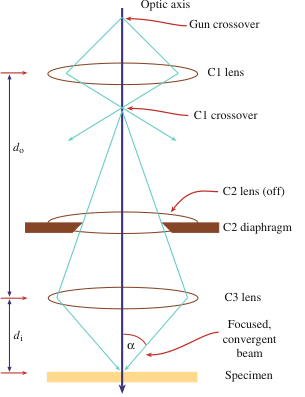
\includegraphics[width=0.5\textwidth, keepaspectratio]{resources/Figures/stem_operating.png}
    \caption{Illumination system for convergent beam.}
    \label{fig:stem_operating}
\end{figure}

% \subsubsection{Energy-dispersive x-ray spectroscopy}
% %Pagina 581 W\&C
% \begin{minipage}[h]{0.6\linewidth}
%         \def\svgwidth{0.66\linewidth}
%         \import{resources/Figures}{Titan_full_column.pdf_tex}
%         \captionof{figure}{Cross-section of an aberration corrected electron microscope}
%         \label{fig:tem_crossection}
% \end{minipage}


\subsection{Crystallography of Transition Metal Dichalcogenides (TMDs)}
\subsubsection{Transition metal dichalcogenides}
Transition metal dichalcogenides or TMDCs are a family of materials consisting of transition metals (group 3 through 12 on the periodic table) and chalcogen atoms (Sulphur, Selenium or Tellurium) in an \ce{MX_2}-configuration, where \ce{M} is the metal atom and \ce{X_2} are the chalcogen atoms \cite{C7TA04268J}.
The properties of TMDCs depend greatly on the amount of stacked layers and with individual layers being as thin as \SI{6.5}{\angstrom} for \ce{MoS_2} these materials are often referred to as layered or two-dimensional materials.
Decreasing the amount of layers from bulk changes electrical properties such as the bandgap which for some TMDCs can go from an indirect to a direct bandgap.
These electrical properties make TMDCs useful in electronics as transistors and in optoelectronics as emitters and detectors \cite{emerg_photolum, LopezSanchez2013, Radisavljevic2011}. 
If present, multiple layers of TMDCs are held together by weak interlayer Van der Waals forces making these materials flexible and transferable using polymer based techniques \cite{reganEmergingExcitonPhysics2022a}.

\subsubsection{Crystal lattice}
An infinitely repeating group of atoms is called an ideal crystal, such a crystal is constructed by attaching the same group of atoms, often called a unit cell, to a lattice.
The lattice can be constructed from $n$ independent lattice vectors. $n=1$ for an atomic chain, $n=2$ for a two-dimensional monolayer, and, $n=3$ for a three-dimensional crystal.
If no smaller repeating group of atoms can be constructed to fill the lattice then this group of atoms is called the primitive unit cell and the $n$-independent lattice vectors are then called the primitive translation vectors $a_{n}$ \cite{Kittel1995-qt}.
Each of the $n$ lattice vectors signifies a direction and length of displacement needed such that the shifted crystal lattice is indistinguishable from the original crystal lattice \ref{eq:lattice_equivalent}.
Lattice vectors are also used to specify the orientation of a crystal plane by denoting where the plane intersects the lattice vectors, this procedure allows for unique indexing of crystallographic planes. The use of these planes will be discussed in \ref{sec:diffraction}.
\begin{equation}
    \vec{r}' = \vec{r} + u_1 \vec{a_1} +u_2 \vec{a_2} + u_3 \vec{a_3}
    \label{eq:lattice_equivalent}
\end{equation}

\subsubsection{Reciprocal lattice and electron diffraction}
\label{sec:diffraction}
In the previous section the crystal lattice was introduced, and it was mentioned that there were unique planes characterized by the points where they intersect the lattice vectors.
In reciprocal space every lattice point is equivalent to one set of these planes.
To best understand a crystal, it is helpful to conceptualize it as having two lattices. The first lattice pertains to the organization of the atoms within the crystal's unit cells. The second lattice is a pattern of points that is specific to each crystal and does not correspond to the atom arrangement. Rather, each point in the lattice is linked to a particular set of planes within the crystal \cite{Williams2009-ww}.
Both lattice constructions are equally valid but are helpful under different circumstances; the reciprocal lattice, for instance, is a useful geometrical construct when talking about diffraction.

The reciprocal lattice, just like the crystal lattice, is constructed by vectors; in the case for the reciprocal lattice these are the reciprocal lattice vectors $\vec{b}_n$.
The reciprocal lattice vectors are constructed from the real-space lattice vectors using equation (\ref{eq:lattice_ortho_norm}) and satisfy relation (\ref{eq:lattice_vec_prop}) with their real-space counterpart.
Using these definitions the reciprocal lattice vectors are unique.
Any reciprocal vector can now be composed uniquely by a linear combination of the reciprocal lattice vectors, such that any vector is scaled and summed. If the scalars are integers they are the miller indices and correspond to a crystallographic plane. \\
Scattering off of these planes shows as a series of high-intensity spots in a diffraction pattern image (Figure \ref{fig:diffraction_pattern}), such an image can be taken in the diffraction mode of a scanning transmission electron microscope (STEM). \\

\begin{minipage}{0.5\textwidth}
    \begin{equation}
        \vec{b}_i = 2 \pi \vec{a}_j \times \vec{a}_k \cdot \left[ \vec{a}_i \cdot ( \vec{a}_j \times \vec{a}_k ) \right]^{-1} 
        \label{eq:lattice_ortho_norm}
    \end{equation}
\end{minipage}%
\begin{minipage}{0.5\textwidth}
    \begin{equation}
        \vec{b}_i \cdot \vec{a}_j = 2\pi \delta_{ij}
        \label{eq:lattice_vec_prop}
    \end{equation}
\end{minipage}\\

In a transmission electron microscope the electrons emanating from the field emission gun are modelled as plane waves. When incident on an atomically thin crystalline sample, the plane waves scatter predictably following the physical criteria that incoming and outgoing electrons beams are plane waves with wave vectors $\vec{k_I}$ and $\vec{k_O}$ for incoming and outgoing waves. The resulting change in wave vector due to the scattering of the sample is then equal to $\vec{K} = \vec{k_I}-\vec{k_O}$. As seen in Figure \ref{fig:scatt_angle}, the outgoing electron beam wavefront is deflected by an angle $\theta$ from the incident electron beam such that both are in phase, this angle is the Bragg angle \cite{Williams2009-ww}; and using that $\vert \vec{k_I} \vert = \vert \vec{k_O} \vert = \vert \vec{K} \vert =\lambda_e^{-1}$, with $\lambda_e$ the electron wavelength, the scattering angle can be expressed as:

\begin{equation}
    \sin{\theta}=\frac{\vert \vec{K}\vert / 2}{\vert \vec{k_I}\vert}
    \label{eq:bragg_angle}
\end{equation}

If both outgoing rays from the same incoming beam wavefront are then in phase, meaning that the extra distance travelled by on of the rays is a multiple of the wavelength, it shows as a bright spot in the image and then the following condition is met for the Bragg angle:

\begin{equation}
    n \lambda_e = 2 d \sin{\theta_B}
    \label{eq:bragg_angle_ser}
\end{equation}

This shows that scattering allows for a finite quantized momentum transfer from the electron to the crystal lattice or vice versa. In a crystalline sample this results in bright spots in the diffraction image, where each bright spot can be indexed and attributed to a family of planes in the crystal that facilitate the momentum transfer for the electrons to reach that spot on the detector or phosphor film.
Just as the real-space lattice has a unit cell so does the reciprocal lattice. In reciprocal space this unit cell is called the Brillouin zone.

\begin{figure}
    \centering
    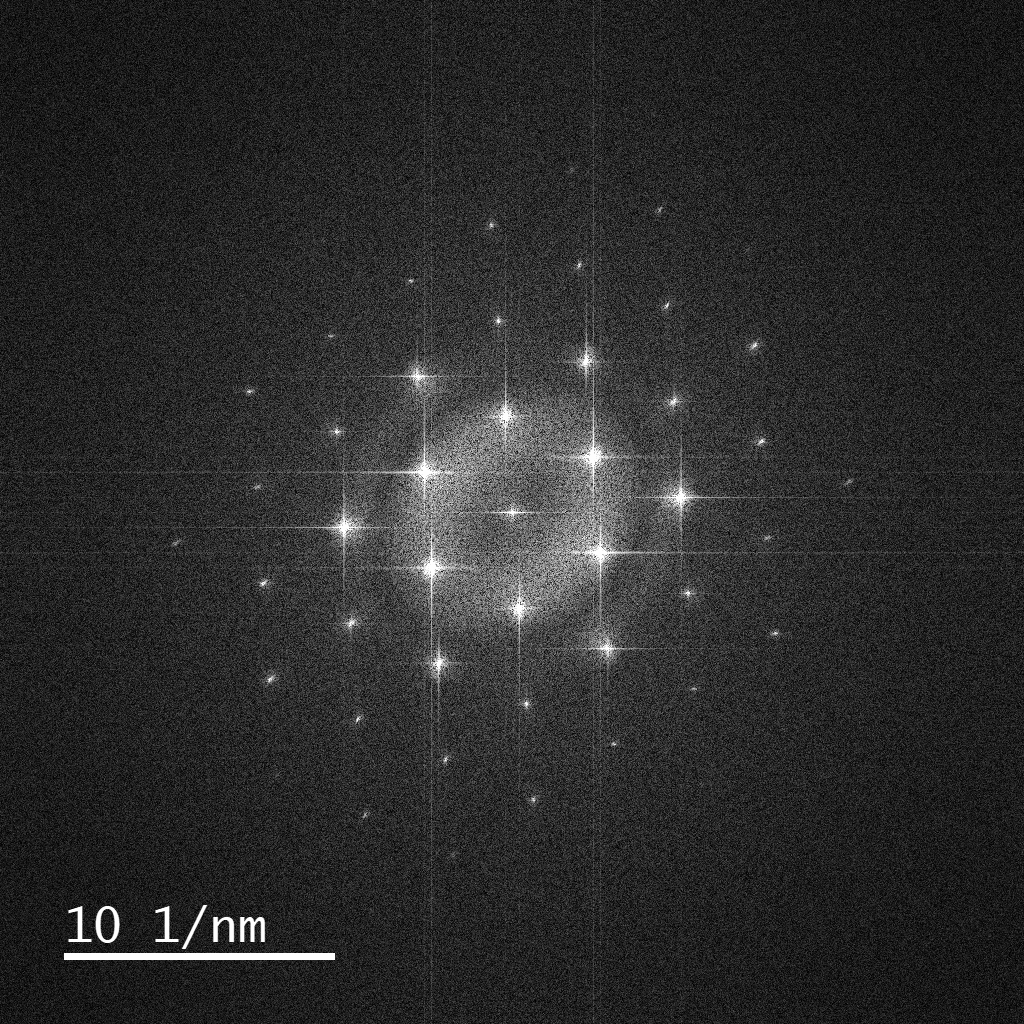
\includegraphics[width=0.3\textwidth, keepaspectratio]{resources/Figures/fft_of_ml.png}
    \caption{Diffraction Pattern}
    \label{fig:diffraction_pattern}
\end{figure}

\begin{figure}
    \centering
    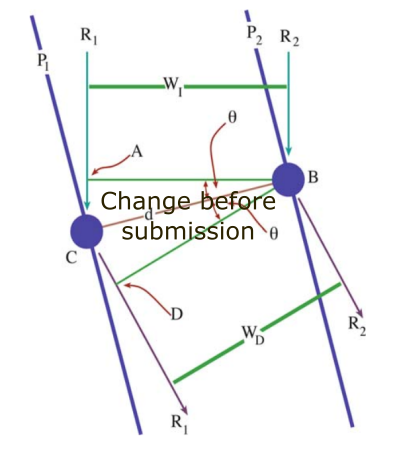
\includegraphics[width=0.3\textwidth, keepaspectratio]{resources/Figures/scattering.png}
    \caption{Scattering diagram}
    \label{fig:scatt_angle}
\end{figure}

\subsubsection{Convergent beam electron diffraction}
In convergent beam electron diffraction the sample is not illuminated by a parallel beam of electrons but instead the electron microscope forms a cone-like shape such that all electrons are focused onto a area only a few atoms wide. The convergence of the electron beam is characterised by the semi-convergence angle $\alpha$ and is usually few to tens of \si{\milli\radian} in size.
Since the local crystal structure is now imaged by a cone-like probe, and not a parallel beam, it is illuminated from multiple different incoming angles; this distribution of incoming angles is then scattered due to the planes in the crystal lattice with the effect of opening the Bragg spots from the previous section to Bragg disks. A typical CBED pattern is displayed in Figure \ref{fig:pacbed}.

\begin{figure}
    \centering
    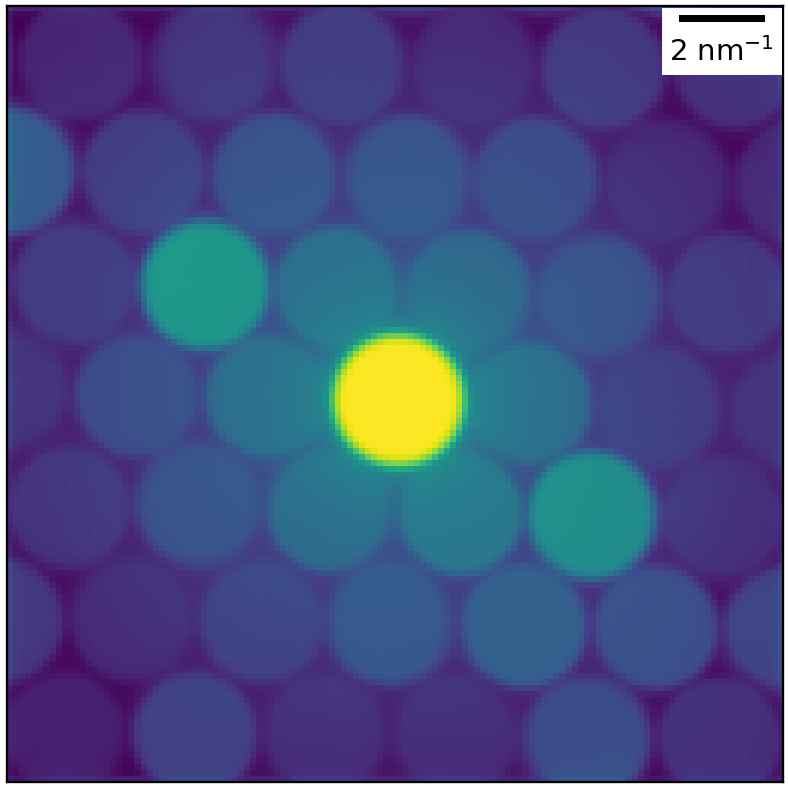
\includegraphics[width=0.5\textwidth, keepaspectratio]{resources/Figures/pacbed_hole.png}
    \caption{A convergent-beam electron diffraction pattern imaged using the EMPAD sensor. Image was calibrated by determining the distance in pixels between Bragg disks and comparing to the FFT of the same crystal imaged using the calibrated CETA camera.}
    \label{fig:pacbed}
\end{figure}

\subsection{Moiré Physics in two-dimensional heterostructures}

\begin{figure}[h]
    \centering
    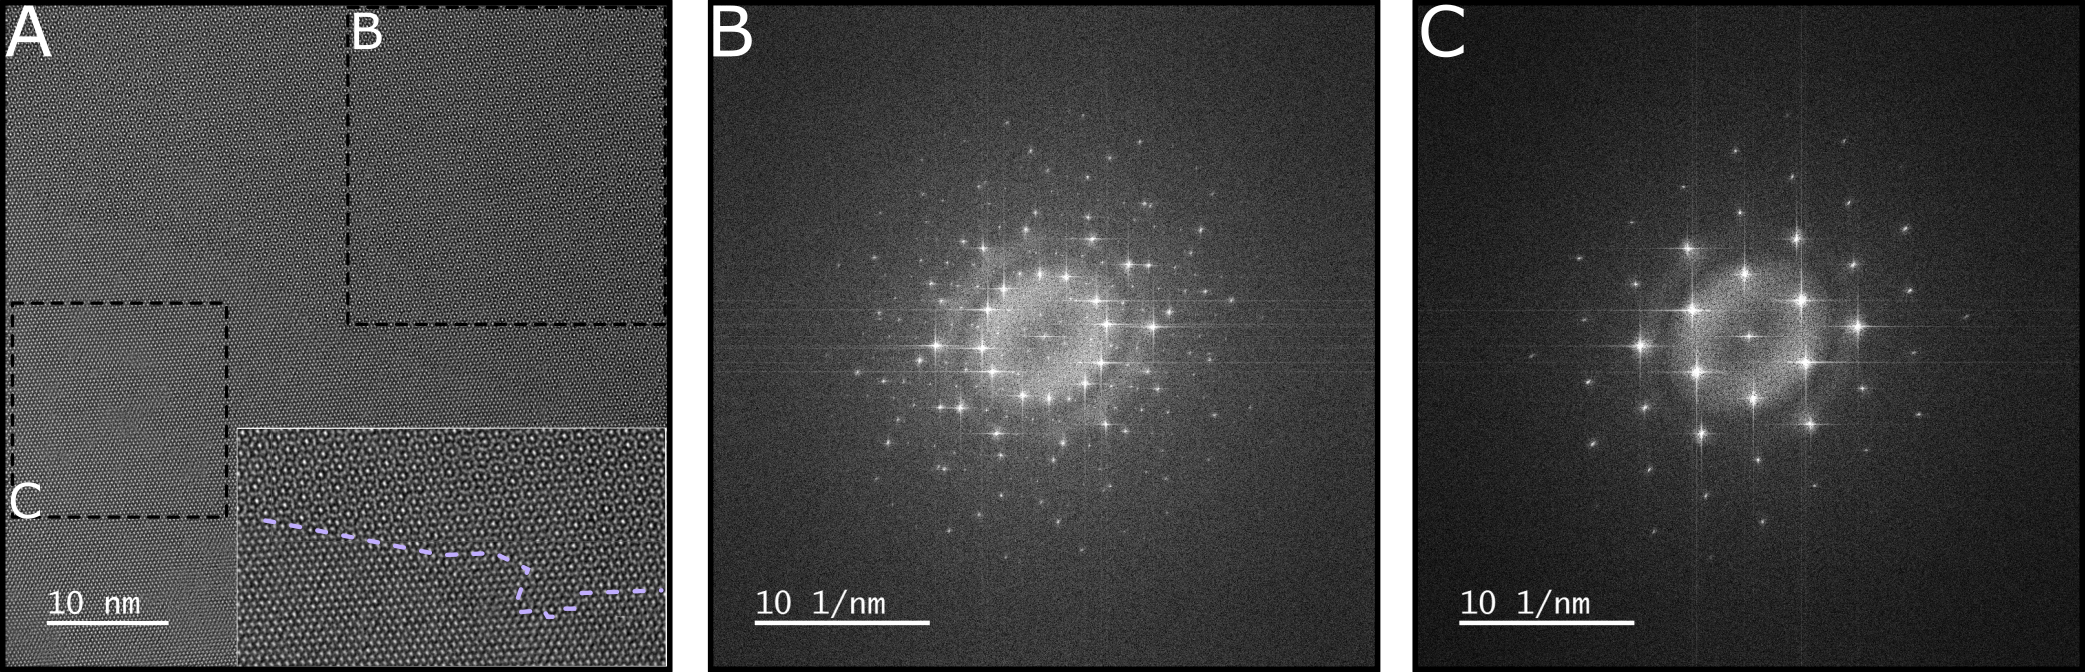
\includegraphics[width=1\linewidth, keepaspectratio]{resources/Figures/moire_transition.png}
    \marginnote{Check detail of Figure \ref{fig:moire_trans}A in print, maybe switch with larger moiré cell} 
    \caption{\textbf{a} High-resolution TEM image of a transition region between singular TMDC material and a twisted heterostructure showing the smallest possible moiré supercell. Dashed regions correspond to subfigures of the same letter, the with white outlined inset is a post-measurement zoomed in image of the transition region with a dashed line guiding the eye towards the flake edge that causes the visual transition. \textbf{b,c} Fast-Fourier transforms of the dashed regions in \textbf{a}. \textbf{b} Shows twelve first-order diffraction peaks indicating that this region consists of two different layers with a roughly \SI{30}{\degree} twist, leading to the smallest possible moiré cell. \textbf{c} Shows six first-order diffraction peaks indicating that its from a single untwisted  crystal. }
    \label{fig:moire_trans}
\end{figure}

Interaction between imaging electrons and crystal lattices lead to the effects described in the previous section, adding a second crystalline structure rotated with respect to the first will affect both lattices as well as create a larger also periodic moiré lattice.
Figure \ref{fig:moire_trans}\textbf{a} shows the transition from single crystal layer to a bilayer region where the constituent layers are rotated from one another, in this bilayer region the effective enlargement of periodic structure is visible as the repeating moiré unit cell is significantly larger than the periodic unit cell of the single layer. The periodicity of the moiré cell is dependent on the rotation between layers and is smallest for \SI{30}{\degree} rotation and increases as the rotation is decreased. The exact periodicity depends on the combination of materials but can be as large as tens of nanometres for transition-metal dichalcogenides with small lattice mismatch \cite{rosenbergerAtomicReconstructionMoire}.

\subsubsection{Diffraction patterns of moiré heterostructures}
The diffraction patterns displayed in Figure \ref{fig:moire_trans}\textbf{b,c} corresponding to the moiré region and the single layer region in Figure \ref{fig:moire_trans}\textbf{a} respectively share some peaks but not all and the extra peaks can not be explained by rotating the diffraction pattern in Figure \ref{fig:moire_trans}\textbf{c} and superimposing in on the pattern in Figure \ref{fig:moire_trans}\textbf{b}.
These extra satellite peaks that emerge between the main Bragg spots and surround the central spot are attributed to the electrons scattering twice, once of off the first layer and then a second time of off the second layer, transferring momentum between the layers while doing so. As these satellite peaks are second order effects they appear dimmer than the main Bragg diffraction spots.
These extra momenta transfer possibilities that open up are displayed schematically in Figure \ref{fig:moire_saed}. In Figure \ref{fig:moire_saed}\textbf{a} the diffraction patterns of two crystal lattice, one red and one blue, are presented; these two lattices each allow six first order momenta transfers by themselves but when brought into proximity the second layer allows scattered electrons to scatter again of its lattice creating the compounded scattering vectors displayed in orange in Figure \ref{fig:moire_saed}\textbf{a,b}. In Figure \ref{fig:moire_saed}\textbf{c} a moiré diffraction pattern is indexed by the cause of the peaks.


\begin{figure}[h]
    \centering
    \def\svgwidth{1\linewidth}
    \import{resources/Figures}{moire_saed.pdf_tex}
    \caption{\textbf{a} Schematic of diffraction patterns of two crystalline samples (red and blue) with a relative twist. The vectors: $\vec{r}_i^n$, $\vec{b}_i^n$, $\vec{c}_i^n$, illustrate the momentum transfers possible due to scattering of a family of planes in the red, blue, or, compound crystal; respectively. In the notation $n$ and $i$ denote the order and the cluster within that order. \textbf{b} Illustration highlighting the new momentum transfer possibilities that open up as two twisted crystalline samples are brought into contact. The newly formed satellite peaks are linear combinations of the intracrystal momentum transfers allowed by the red and/or blue crystal structure and an intercrystal momentum transfers. \textbf{c} Schematic overlaid onto the FFT of a HRTEM image of a moiré cell.}
    \label{fig:moire_saed}
\end{figure}


\newpage
\section{Fabrication of two-dimensional (2D) Moiré heterostructures}
\label{sec:fab_method}
%
%Start the chapter with a brief introduction that outlines the importance of fabricating 2D Moire heterostructures and their relevance to your research.

% 2d mat. promising for future applications 
% hughe degree of custimisability with strain- twisttronics and choice of material
% engineering perfect meta-material for application specific needs
% Stamping allows for fast prototyping

The fabrication process of 2D Moir\'e heterostructures plays a pivotal role in determining the properties and performance of these structures. In this thesis, we refer to this process as 'mechanical transfer', where two monolayers are stamped together to form a bilayer heterostructure. This step significantly influences the properties and performance of these structures. 
%
Through the 'mechanical transfer' process, we gain control over important parameters such as layer thickness, orientation, and lattice mismatch of individual layers, which are key factors in determining the interference pattern and the overall properties of the heterostructure.

In the following, I will explain the step-by-step process we followed to fabricate these structures. This includes exfoliating single layers, verifying their thickness, assembling them, and transferring them to a specialised microscope.


\subsection{Exfoliation of monolayer material}
%
For the preparation of the heterostructures, monolayer flakes were prepared using a three-step process.
%
First, the bulk crystal material was exfoliated two to three times between Scotch tape, using the same method commonly used for graphene~\cite{novoselovRoomTemperatureQuantumHall2007}. 
%
These flakes were then transferred to a polydimethylsiloxane (PDMS) stamp.
%
This was done by placing the PDMS stamp on the Scotch tape with the flakes and then quickly peeling the stamp off with tweezers. 
%
It is important to note that for PDMS, the adhesion force to the flake is proportional to the peel-off speed~\cite{kusakaMicrocontactPatterningConductive2015}.
%
Third, the flakes present on the PDMS stamp were inspected using an optical microscope before being exfoliated using PDMS stamps. At this stage, PDMS stamps are used for exfoliation, as they provide a gentler way of further cleaving the bulk flakes and eliminating a further transfer step from tape to PDMS if a monolayer flake were to be exfoliated using tape since stamping on a substrate with tape is difficult. The exfoliation using two PDMS stamps is performed by laying the stamps on another while on a glass slide to provide support, after which both stamps are peeled from the glass before separation by two tweezers. Both stamps are now inspected by means of an optical microscope, and if monolayer (ML) material is present on either of the stamps it can later be used in creating a heterostructure.
If no ML material is present on a stamp, the third step can be repeated until there is ML material or the flakes have broken up into unusable small pieces.
Furthermore, sacrificial or pristine PDMS stamps can be used to either remove unwanted small flakes or transfer large flakes to a newer and cleaner PDMS stamp, and this selective transfer is performed under a microscope such that existing ML material can be avoided as this will likely break if exposed to the force caused by peeling away the sacrificial PDMS stamp.

\subsection{Verification of monolayer material}
\begin{figure}[h]
	\centering
	\def\svgwidth{1\linewidth}
	\import{resources/Figures}{spectroscope_traces.pdf_tex}
	\caption{Transmittance spectra, recorded using a light spectrometer, show flakes of varying thicknesses. A) Transmittance spectra for 1 to 6 layers of $WSe_2$ exfoliated on a PDMS-coated glass substrate using the method described previously. 
    %
    B) Transmittance spectra of 1 to 3 layers of $MoSe_2$.
    %
    C,D) The flakes used to collect the spectra of $WSe_2$ (A, C) and $MoSe_2$ (B,D), respectively.
    %
    In A), the square, circular, and diamond markers denote the location of the peaks of the \textit{a}-,\textit{c}-, and, \textit{d}-exciton of $WSe_2$, found by fitting a linear combination of Lorentzian peaks. The shaded blue region denotes the photon energy range in which the \textit{b}-exciton peaks are expected but not found by the fitting model.
    %
    Similarly, in B), the square and circular marker denote the location of the \textit{a}- and \textit{b}-exciton peaks of $MoSe_2$.}
    %
	\label{fig:spectroscope_traces}
\end{figure}

\begin{minipage}[b]{0.4\textwidth}
    \begin{tabular}{c|cc|}
    \cline{2-3}
    \multicolumn{1}{l|}{}         & \multicolumn{2}{l|}{Photon Energy of  Exciton {[\si{\electronvolt}]}} \\ \hline
    \multicolumn{1}{|c|}{lay. \#} & \multicolumn{1}{c|}{A}                                        & B                                       \\ \hline
    \multicolumn{1}{|c|}{1}       & \multicolumn{1}{c|}{1.54}                                     & 1.79                                    \\ \hline
    \multicolumn{1}{|c|}{2}       & \multicolumn{1}{c|}{1.55}                                     & 1.80                                    \\ \hline
    \multicolumn{1}{|c|}{3}       & \multicolumn{1}{c|}{1.56}                                     & 1.80                                    \\ \hline
\end{tabular}
\captionof{table}{Measurements of the dip positions for the A- and B-exciton in $MoSe_2$ flakes of varying layer thickness}
\label{tab:mose2_measurement_spectra}
\end{minipage}%
\hspace{0.1\textwidth}%
\begin{minipage}[b]{0.4\textwidth}
    \begin{tabular}{c|ccc|}
    \cline{2-4}
    \multicolumn{1}{l|}{}         & \multicolumn{3}{l|}{Photon Energy of  Exciton {[\si{\electronvolt}]}} \\ \hline
    \multicolumn{1}{|c|}{lay. \#} & \multicolumn{1}{c|}{A}                   & \multicolumn{1}{c|}{C}                  & D                  \\ \hline
    \multicolumn{1}{|c|}{1}       & \multicolumn{1}{c|}{1.666}               & \multicolumn{1}{c|}{2.429}              & 2.813              \\ \hline
    \multicolumn{1}{|c|}{2}       & \multicolumn{1}{c|}{1.654}               & \multicolumn{1}{c|}{2.323}              & 2.742              \\ \hline
    \multicolumn{1}{|c|}{3}       & \multicolumn{1}{c|}{1.644}               & \multicolumn{1}{c|}{2.226}              & 2.716              \\ \hline
    \multicolumn{1}{|c|}{4}       & \multicolumn{1}{c|}{1.632}               & \multicolumn{1}{c|}{2.200}              & 2.726              \\ \hline
    \multicolumn{1}{|c|}{5}       & \multicolumn{1}{c|}{1.623}               & \multicolumn{1}{c|}{2.200}              & 2.820              \\ \hline
    \multicolumn{1}{|c|}{6}       & \multicolumn{1}{c|}{1.622}               & \multicolumn{1}{c|}{2.182}              & 2.794              \\ \hline
\end{tabular}
\captionof{table}{Measurements of the dip positions for the A-, C- and D-exciton in light transmittance spectra of $WSe_2$ of varying thickness.}
\label{tab:wse2_measurement_spectra}
\end{minipage}
\vspace{1cm}

Since the bandgap of TMDCs becomes direct in a single layer,the  and most interesting moir/'e effects come into play for monolayer flake heterostructures, it is important to determine the number of layers in the flakes used for heterostructures. 
For the first round of samples, optical inspection with a transmittance light microscope proved to be too crude to determine the layer number for flakes thinner than three layers.

Solving this issue involved setting up a new transmittance- and reflectance-mode microscope with a spectroscope attached. The entire setup was copied from another lab and has been proven capable of differentiating between the number of layers in a flake~\cite{frisendaMicroreflectanceTransmittanceSpectroscopy2017,niuThicknessDependentDifferentialReflectance2018}.

Using this setup, we recorded transmittance and reflectance spectra for both $WSe_2$ and $MoSe_2$ flakes with varying layer numbers.
%
The transmittance spectra are displayed in Figure~\ref{fig:spectroscope_traces}A for $WSe_2$ and Figure~\ref{fig:spectroscope_traces}B for $MoSe_2$. 
%
While both transmittance and reflectance spectra should ideally have used the same halogen bulbs for illumination in both transmission and epi-illumination modes, the reflectance spectra exhibited more noise in the energy range of $\leq \SI{1.6}{\electronvolt}$ due to the lower intensity emitted by the epi-illumination bulb in this region. As a result, we omitted the reflectance spectra from this study.

All spectra were collected using a $100\times$-magnification $0.55NA$ objective, along with a \SI{150}{\micro\meter} thick core glass fiber leading to the spectrometer. 
%
The spectrometer collected and averaged 50 spectra, which were integrated over \SI{500}{\milli\second}. To improve the rejection of stray light, the field aperture of the light was fully closed.

As can be seen in the transmittance spectra, the overall intensity difference is the best indicator for flake thickness beyond 2 layers, whereas the location of the A-exciton is the key differentiator between 1 or 2 layers. 
%
Using the spectroscope and the new microscope has greatly reduced the time required and greatly improved the ease of finding thin material and verifying its thickness.

\subsection{Assembling a heterostructure}
\begin{figure}[h]
	\centering
	\def\svgwidth{1\linewidth}
	\import{resources/Figures}{stamping.pdf_tex}
	\caption{Schematic outline of the stamping process. 1: Before starting, two PDMS stamps with monolayer material and a silicon substrate coated with PVA should be prepared. 2: The first flake is stamped, preferably as close to the centre of rotation of the substrate stage as possible as this makes aligning the next flake easier. 3: The micromanipulator with the PDMS stamp is slowly raised to peel the PDMS stamp off of the substrate, leaving behind the first monolayer flake. 4: The second stamp with monolayer material is aligned by rotating the substrate stage and moving the stamping micromanipulator. 5: The stamp is then carefully lowered and misalignment is corrected if necessary. 6: The second stamp is removed slowly, and both flakes are transferred to the substrate.}
	\label{fig:stamping_process}
\end{figure}

Once two suitably matching monolayer flakes have been located on different PDMS stamps they can be assembled to form a heterostructure.
The flakes are stamped onto a specially prepared substrate using a dedicated stamping set-up that allows for micrometer precise control over flake position and consists of two main parts: a substrate stage, and, a flake stage.
The substrate stage has three degrees of freedom: two micromanipulators control the $x$- and $y$-position of the substrate under the microscope and the stage itself is free to rotate to align the edges of the to be stamped ML flakes.
The stamping stage is capable of precisely moving a glass slide with a stamp along three axes.
The complete stamping set-up is pictured in Figure \ref{fig:stamping_set-up} and is a direct adaptation from previously published set-ups \cite{castellanos-gomezDeterministicTransferTwodimensional2014, castellanos-gomezDeterministicTransferTwodimensional2014a}.
The stamping set-up consists of: a reflective optical microscope, a rotating substrate stage attached to two micromanipulators, and, a stamping stage connected to three micromanipulators.
The ML material is stamped onto the substrate by first adhering the PDMS stamp onto a glass microscope slide and inserting this slide into a holding mechanism on the stamping stage, after which the stamp is carefully brought into contact with the substrate as illustrated in Figure \ref{fig:stamping_process}.
Since we wish for the flake to adhere to the substrate and not the stamp, we now slowly release the stamp from the substrate, the stamp peel-off speed is crucial at this step and should be as slow as possible without stopping the process.
During this step of the process it is also paramount to not introduce any vibration or other forces as these can easily tear the flake.
\begin{figure}[h]
	\centering
	\def\svgwidth{1\linewidth}
	\import{resources/Figures}{stamping_setup.pdf_tex}
    \caption{Photograph of the stamping set-up used to stamp heterostructures on a polymer coated diced silicon wafer. From the top to the bottom of the set-up denoted are: A camera which is connected to an adjacent computer to provide a live view of the process, a variable $\times$2\--$\times$12  zoom lens, a glass fibre coming from a halogen source (not pictured) for epi-illumination of the process, a piece of carbon tape used for holding the diced silicon chip, the micromanipulators used for positioning the silicon substrate and potential flake, a glass slide with a PDMS stamp and flake, and, the micromanipulators used to position the stamp.}
	\label{fig:stamping_set-up}
\end{figure}

Applying the second stamp with ML material requires more care and effort as this stamp needs to be aligned with the first already stamped monolayer flake. The aligning step is performed by first locating the ML material on the substrate and then roughly aligning the micromanipulator with the second flake. Then experience has shown that the easiest way to proceed is by aligning the edges of both flakes to the desired angle as changing the angle of the flake on the substrate requires rotating the stage and most likely the stamped flake out of view. After alignment of the angles it is now possible to place the flakes above one-another using the micromanipulators. Slowly lowering the second stamp to the substrate will bring both flakes into view allowing for a more precise alignment, during further lowering of the flake its best to zoom out as to be able to see where the PDMS stamp first contacts the substrate. If this first point of contact is too far from the ML material, further lowering of the stamp can squeeze the PDMS and cause the flake to move in the direction of the contact-front propagation during further lowering; if this happens restarting the stamping procedure and compensating for the movement is possible, but it is advised to remove the glass slide with the flake completely and cut the PDMS in such a way that the first point of contact is closer to the ML material.
After stamping of the second flake is completed the PDMS needs to be slowly peeled of again in the same manner as before, after which the result will be a heterostructure on the prepared substrate, ready for transfer to a TEM grid.

\subsection{Transferring to a TEM grid}
\begin{figure}[h]
	\centering
	\def\svgwidth{1\linewidth}
	\import{resources/Figures}{wet_transfer.pdf_tex}
	\caption{Schematic illustration of the transfer process. 1: A previously prepared heterostructure is located on the substrate and suitable TEM grid is placed on the substrate over the heterostructures with tweezers. 2: The TEM grid is held in place, for the samples transferred for this work the TEM grid was held in place by pressing a microscope slide onto the rim of the TEM grid with the stamping micromanipulator taking care in not pressing too hard as this will push the TEM grid into the PVA sealing the inside in such a way that the IPA cannot reach the inside. 3: After wetting the grid with a drop of IPA the resulting surface tension will hold onto the carbon film as the drop evaporates pulling it onto the PVA coated substrate and heterostructure. 4: After all the IPA has evaporated and the glass slide is removed a single drop of distilled water is added to dissolve the PVA releasing the TEM grid and allowing it to float on the drop, ready to be picked up with tweezers.}
	\label{fig:wet_transfer}
\end{figure}

Transfer of the heterostructure to a TEM grid was performed using a previously devised polymer assisted method \cite{kosterPolymerassistedTEMSpecimen2021}, where a diced silicon wafer is coated using a polymer before stamping.
The flakes are then stamped directly on the polymer coating in the same manner as described in the previous section before being covered with a TEM grid, application of a single drop of either water or IPA  depending on the polymer used connects the flexible holey carbon film of the TEM grid with the polymer coating by means of surface tension as the drop evaporates. This "seals" the heterostructure in between the holey-carbon film and the polymer.
Adding another drop, this time the solvent for the polymer, allows the flake held by the TEM grid and the grid itself to separate from the silicon substrate; allowing it to be picked up using tweezers.
The process is illustrated in Figure \ref{fig:wet_transfer}.
The authors of the previously cited paper demonstrated that both the use of PMMA and PVA are possible but require different solvents, acetone and water respectively.
The heterostructures transferred for this thesis were stamped on a diced silicon wafer coated with \(\sim \) \SI{100}{\nm} thick PVA and were then annealed at \SI{400}{\degreeCelsius} in vacuum as there was significant contamination present.

\newpage
\section{Four-Dimensional Scanning Transmission Electron Microscopy (4D-STEM) technique for mapping Moiré physics at the nanoscale}

\subsection{Electron microscope pixel-array detector}
%In TEM operating mode a parallel electron beam is used to illuminate the sample and form an image on either the phosphorous screen or digital camera, this spreads the beam over a larger area such that the local electron dose is relatively uniform.

%-------------------------------------------------------
\begin{figure}[h]
	\centering
	\def\svgwidth{0.65\linewidth}
	\import{resources/Figures}{empad-haadf.pdf_tex}
	\caption{The figure schematically shows the difference between a monolithic fixed geometry high-angle annular dark field (HAADF) detector and a pixelated-array detector on the left- and right-hand side of the image respectively. 
    %
    As shown, the HAADF detector is only able to resolve features whose scattering diffracts the beam onto the monolithic annular detector. Since the Bragg angle is fixed for each feature, the signal can only be captures at a certain camera length. 
    %
    The HAADF detector is a single large punctured "pixel" that bunches all incident signals together.
    %
    In contrast, the EMPAD is able to capture signals diffracted over a wider range of angles for every camera length as well as spatially separate the different signals, a HAADF and bright field detector could then be simulated by virtually masking and integrating the equivalent regions of the data after a measurement.}
	\label{fig:empad_haadf_comparison}
\end{figure}
%-------------------------------------------------------

The electron microscope pixel-array detector (EMPAD),  is as the name suggest a sensor for electron microscopes that consists of a grid of direct electron detecting pixels. 
%
Even though the EMPAD can be used in standard transmission electron imaging its strengths lie in scanning-TEM imaging due to the relatively little pixels but greater dynamic range of said pixels.
%
In a scanning-TEM (STEM) mode the beam is cone-shaped and converges to a thin point-like spot that scans over the specimen, for small semi-convergence angles the zeroth order diffraction disk is a magnitude higher in intensity than the first order Bragg reflection disks.
%
Since there is valuable information in the distribution of intensity in all disks its important that the detector has sufficient dynamic range to count individual electrons at all intensity ranges simultaneously using a high-gain per pixel charge integration circuit. 
%
The second major advantage of the EMPAD is the pixelated-array of detectors that, contrary to the regular monolithic annular dark field detectors, preserves the deflection angle information of the transmitted electron beams.
%
Traditionally, elastic scattering deflects the electrons from the optical axis onto one of the annular ring shaped detectors encircling the optical axis, these detectors are called the dark field detectors.
%
These singular annular detectors have a fixed detector geometry that only captures signals at certain camera lengths when diffracted beams are impinging on the detector, as schematically shown in Figure \ref{fig:empad_haadf_comparison}. 

The EMPAD solves this problem by measuring the whole convergent-beam electron-diffraction (CBED) pattern using a single fast-readout, high dynamic range pixel grid on which every pixels' electron dose is stored separately such that after acquisition of a complete STEM scan the bright- and dark-field detectors can be virtually recreated by integrating the electron dose using annular or circular masks on the data.
%
The pixelated nature of the detector enables the precise computation of the intensity distribution of not only the whole CBED pattern but also within each diffraction disk within the CBED pattern, greatly improving the potential resolution by means of ptychography methods \cite{pennycookEfficientPhaseContrast2015, yangEfficientPhaseContrast2015a} as well as enabling charge density analysis \cite{hachtelSubAngstromElectricField2018,wenMapping1DConfined2022,fangAtomicElectrostaticMaps2019} and strain analysis \cite{hanStrainMappingTwoDimensional2018, ophusFourDimensionalScanningTransmission2019}.
%
The EMPAD's sensor is made up of a grid of 128 by 128 pixels and will thus always image the CBED or NBED pattern at this resolution. 
% SC, move this up

%
Every pixel counts single electron charges and stores the count in a 32-bit number. 
%
The EMPAD is able to equal the field-of-view of the HAADF-detector with a maximum of 512 by 512 equally positioned scan points. 
%
A schematic showing the geometry of a measurement is given in Figure \ref{fig:4d_dataset}a where a scanning probe is shown to scan over a diamond shaped Moiré unit cell creating a CBED pattern on the EMPAD's pixel-array sensor. 
%
Nine CBED patterns for differing probe positions are displayed in Figure \ref{fig:4d_dataset}b. By virtually masking and integrating the first-order Bragg reflections for every CBED pattern to a single electron count one is able to recover a virtual annular dark-field image. % SC, define first-order bragg

%-------------------------------------------------------
\begin{figure}[h]
	\centering
	\def\svgwidth{1\linewidth}
	\import{resources/Figures}{4d-dataset.pdf_tex}
	\caption{\textbf{a}) Schematic overview of an EMPAD measurement where a convergent electron beam probes the sample at positions $\vec{r}_1$ through $\vec{r}_5$ producing convergent-beam electron diffraction (CBED) pattern images of 128 by 128 pixels for each such position.\textbf{b}) Nine such CBED patterns imaged at different positions within a moiré cell using electric field measurement conditions.\textbf{c}) A virtual annular dark field image made by masking a thin annulus in the 4d-dataset. With only the first order Bragg reflections captured by the mask the atomic periodicity is visible within the image.}
	\label{fig:4d_dataset}
\end{figure}
%-------------------------------------------------------

\subsection{Strain analysis}% State of the art
%
Strain analysis in electron microscopy can be achieved through a multitude of ways, the main distinction between all of them is whether they are performed by analysing a real-space image captured by high-resolution TEM techniques or performed by analysing reciprocal space images captured through scanning-TEM techniques. 
%
An example of the first method is Geometric Phase Analysis (GPA) where displacements of atoms in a crystal are directly observed in the high-resolution image and strain can be computed \cite{HYTCH1998131, hytchGEOMETRICPHASEANALYSIS1997, nguyenAtomicDefectsDoping2017}. 
%
The second method relies primarily on the fact that a CBED/NBED pattern for a small enough convergent electron probe directly measures the local crystal structure. 
%
The reciprocal-space unit cell of the local crystal structure and thus the positions of the peak in the CBED pattern are directly correlated with the size of the real-space unit cell such that a compressing force in the real-space unit cell will elongate the reciprocal-space unit cell in the same direction and vice-versa for a tensile strain \cite{ophusFourDimensionalScanningTransmission2019, vanwinkleRotationalDilationalReconstruction2023, kazmierczakStrainFieldsTwisted2021, hanStrainMappingTwoDimensional2018}, tracking the peaks then gives access to the strain information.  In the following sections the second method will be applied for both large and small field-of-views.

\subsubsection{Micrometre field-of-view strain analysis}
%
%-------------------------------------------------------
\begin{equation}
	PC\{f(t)\} = \left| \mathscr{F} \left\{ \ln{\left| \mathscr{F}\{f(t)\} \right|^2} \right\} \right|^2
	\label{eq:cepstrum}
\end{equation}
%-------------------------------------------------------

Strain analysis at the micrometre-scale hinges on capturing clear convergent- or nano-beam electron diffraction patterns as the locations of the peaks therein hold the valuable crystallographic information and the by strain induced deviation thereof, thickness and local sample tilt affect the intensity distributions of the patterns in such a way that tracking the peaks over micrometre distances is challenging. % SC show this with an image
%
The average distance between folds, wrinkles, or, the sides of holes in the lacy carbon grids is typically smaller than a micrometre-scale field-of-view; these features tilt the crystalline sample such that the optical axis of the electron microscope is no longer parallel to the crystal zone-axis. Overcoming the effects of local tilt, wrinkles, folds, and, multilayeredness found in stamped heterostructures is achieved by implementing a power cepstrum transform before peak tracking.
%
The power cepstrum transform (equation \ref{eq:cepstrum}) was originally developed for speech analysis \cite{1570854175999207936, oppenheimDspHistoryFrequency2004,nollCepstrumPitchDetermination1967} and later adapted for application to the post-specimen electron exit-wave ($\psi(\mathbf{q})$) whose magnitude is directly probed by the EMPAD \cite{padgettExitwavePowercepstrumTransform2020} as this is the CBED/NBED pattern.

\begin{alignat}{2}
	I(\vec{q}) &  & = \left| \Phi(\vec{q}) \otimes \left( E(\vec{q}) \cdot \mathcal{O}(\vec{q}) \right) \right|^2 & = \left| \psi(\vec{q}) \right|^2
	\label{eq:cbed_comp}                                                                                                                             \\
	\ArrowBetweenLines*[\downarrow^1\hspace{1cm}]%
	I(\vec{q}) &  & \approx \left|E(\vec{q}) \right|^2 \left|\Phi(\vec{q}) \otimes \mathcal{O}(\vec{q}) \right|^2 &
	\label{eq:cbed_approx}
\end{alignat}

The intensity of the recorded pattern can be described as a convolution between the image of the electron beam probe function in momentum-space ($\Phi(\mathbf{q})$) convoluted with the by the envelope function ($E(\mathbf{q})$) multiplied true object function ($\mathcal{O}(\mathbf{q})$) (equation \ref{eq:cbed_comp}); the envelope function encompasses the intensity attenuation due to local sample tilt and thickness, the true tilt-free object function is a sum of delta-peaks describing the crystal structure in momentum space; such that the result is an attenuated pattern formed by placing an image of the electron-beam probe on each delta-peak. 

As can be seen in Figure \ref{fig:adf_nbed_ewpc}b where the intensity of the disks is suppressed towards the edges of the pattern. Under the ideal conditions used for strain-analysis the probe-image is very small, and the envelope function varies little over the whole pattern resulting in a relatively unvarying offset. Therefore; assumption $\downarrow^1$ states that multiplication by the envelope function after convolution is approximately similar to convolution of the multiplied result, such that the intensity distribution can be rewritten to the form of equation \ref{eq:cbed_approx}. Using this simplification, the definition of the power-cepstrum, and, the knowledge that the CBED/NBED patterns are a mechanically computed Fourier transform of the real-space intensity distribution; the exit-wave power-cepstrum of the CBED/NBED pattern can be written as in equation \ref{eq:cepstrum_unsimp}.

\begin{alignat}{3}
	EWPC_{\psi(\vec{q})} & =\left| \mathscr{F}\left\{\ln{\left| E(\vec{q}) \right|^2}\right.\right. &  & +\left. \left.\ln{\left| \Phi(\vec{q}) \otimes \mathcal{O}(\vec{q}) \right|^2}\right\} \right|^2 & \label{eq:cepstrum_unsimp} \\
	\ArrowBetweenLines*[\downarrow^2\hspace{-2cm}]%
	                     &                                                                          &  & \approx \Phi(\vec{q}) \otimes \ln{\left| \mathcal{O}(\vec{q}) \right|^2}                         &                            \\
	                     & \approx PC\left\{ \epsilon(\vec{x})\right\}+                             &  & \left| \phi(\vec{x})\right|^2 \cdot PC\left\{ o(\vec{x})\right\}                                 & \label{eq:cepstrum_simp}
\end{alignat}

Furthermore, if the ronchigram is well-formed and corrected, and a small aperture is used to select only the centre; the second term in equation \ref{eq:cepstrum_unsimp} can be simplified further if the Bragg-spot separation is larger than the convergence angle of the electron-probe, such that the Bragg disks do not overlap. 
%
This assumption $\downarrow^2$ allows for the separation of the EWPC in to a summation of the power-cepstrum of the envelope function and the power-cepstrum of the crystal-structure information \cite{padgettExitwavePowercepstrumTransform2020}. 
%
Since the envelope function in the CBED/NBED pattern varies slowly over the image and the diffraction Bragg-spots are a high frequency repeating pattern both features occupy a different frequency band in the image, they are thus separated by the power-cepstrum transform. The tilt and thickness information is then transformed to and muddles the centre of the EWPC pattern in Figure \ref{fig:adf_nbed_ewpc}c, the crystal-structure information is well separated and occupies a different section in the image.

%-------------------------------------------------------
\begin{figure}
	\centering
	\def\svgwidth{0.9\linewidth}
	\import{resources/Figures}{adf_cbed_ewpc.pdf_tex}
	\marginnote{TODO: Change the CBED and EWPC in this figure to one of an actually used dataset}
	\caption{\textbf{a}) virtual annular dark-field image reconstructed by masking the dataset such that the detector geometry is equivalent to that of the HAADF-detector. Image is taken at the transition region of monolayer $MoSe_2$ (bottom) to a heterostructure of $MoSe_2$ and $WSe_2$ (top) on a lacy carbon grid. The faint circles in the middle of the image are contamination from inspection in TEM mode. Contamination in STEM mode caused the bright white spots on the left side of the image. \textbf{b}) logarithm of the nanobeam electron-diffraction pattern captured in the heterobilayer region of the image in \textbf{a}. Two sets of six diffraction disks, one set of six for each material, can be seen in the pattern. Due to local tilt of the crystalline layers diffraction disks on one side of the central $000$-disk, in this case the bottom, are brighter than disks on the opposing side. \textbf{c}) Exit-wave power cepstrum (EWPC) transform of the NBED pattern displayed in \textbf{b}. The EWPC pattern does not suffer from unequal intensity distributions. Peaks in the pattern are distinguishable in the EWPC transform.}
	\label{fig:adf_nbed_ewpc}
\end{figure}
%-------------------------------------------------------

Beam conditions optimised for strain analysis at the micrometre-scale need to result in being able to separate the Bragg disk on the EMPAD sensor as well as fitting as many spots within the bright part of the envelope on the sensor by optimising the camera length. Generally a smaller spot size, around 5-6, is used to increase electron brightness and the semi-convergence angle of the electron probe is situated around $\approx$\SI{5}{\milli\radian} to achieve well-defined round disks. 
%
This is achieved using a \SI{10}{\micro\meter} to \SI{50}{\micro\meter} aperture in Probe-L mode on the Titan running at \SI{300}{\kilo\electronvolt}.\marginnote{TODO: Change This.}



\subsection{Centre-of-Mass (COM) Analysis for Potential Field Mapping and Phase Object Retrieval}
%
In the context of electron diffraction, the Bragg condition, as described by Bragg's law, play a crucial role. It states that the interference of waves becomes constructive when the path difference between them is an integer multiple of the wavelength. This fundamental principle leads to the formation of the Bragg diffraction spots or disks, which are the prominent features in the diffraction pattern.

Centre-of-mass (COM) analysis is an innovation approach to potential field mapping and phase object retrieval. 
%
It serves as a continuation of differential phase contrast, where a segmented annular detector is utilised to measure the difference in beam intensity on two pairs of opposing detectors. 
%
This methodology offers valuable insights into the deflection of electrons caused by the sample. 
%
By employing the COM technique, we can effectively  retrieve phase information. 
%
Furthermore, this approach has evolved to accommodate pixelated-array detectors, enabling the capture of the first moment of the electron beam on the detector plane. 

The central Bragg diffraction spot or disk is often described as unscattered, but this is a simplification. 
%
While it is true that the spot/disk is not scattered by the crystal structure, it can be deflected from its  unperturbed position by angles much smaller than the Bragg angles. 
%
This deflections occurs due to the phase acquired by the electrons in the beam during their interaction with electric or magnetic fields.

This shift in position is only detectable when the electron probe is physically much smaller than the electric or magnetic field it interacts with.
%
Conversely,if the probe is much larger than the probed feature, one instead observed a redistribution of the intensity within the bright field disk.
%
Both these scenarios necessitate different analysis processes.

However, they both start from the same assumption: that the electron probe wavefunction $\psi_{in}(\vec{k})$ interacts with a sample that can be modelled as a pure phase object. This interaction only adds a phase component to the incoming wavefunction\cite{caoTheoryPracticeElectron2018, lazicPhaseContrastSTEM2016}. 

The outgoing wavefunction of the electron probe can be described as follows:

\begin{equation}
    \Psi_{out}(\vec{r},\vec{r}_p)=\psi_{in}(\vec{r}-\vec{r}_p)\exp(2\pi i \Delta \vec{k})\\
    \label{eq:out_wav}
\end{equation}

Here, $\vec{r}_p$ denotes the position of the probe, $\Delta k$ represents the phase shift, and, $\psi_{in}$ is the incoming wave modelled as a plane wave. The semi-convergence angle of this plane wave is imposed by an aperture $A(\vec{k})$.

The incoming wave is given by the following equation:

\begin{equation}
    \psi_{in}(\vec{r})=\mathcal{F}^{-1}\left\{A(\vec{k})\exp(i\chi(\vec{k}))\right\}(\vec{r})
    \label{eq:in_wav}
\end{equation}

%\subsubsection{Probe << Features}



%-------------------------------------------------------
\begin{figure}[h]
	\centering
	\def\svgwidth{1\linewidth}
	\import{resources/Figures}{probe_small_features_biig.pdf_tex}
    \caption{\textbf{Left:} When electron probes have crossover areas much smaller than the features being imaged, the entire diffracted outgoing wavefunction is subjected to complete deflection. \textbf{Right:} This deflection becomes evident through a uniform translation on the imaging plane, as indicated by the arrow highlighting the shift from the centre.}
	\label{fig:small_probe}
\end{figure}
%-------------------------------------------------------

In the scenario where the probe's cross-sectional area is much smaller than the feature being imaged, it can be assumed that the sample potential is a linear ramp across the probe's cross-sectional area ~\cite{caoTheoryPracticeElectron2018}. 
%
At the detectors, the magnitude of the Fourier transformed wavefunction is measured. The phase shift in real space is then transformed into a displacement in reciprocal space.
%
The displacement in reciprocal space is linearly dependent on the electric and/or magnetic field. The final diffraction pattern recorded on a sensor in STEM imaging is then given by Equation~\ref{eq:lin_shift}, where $t$ is the thickness of the sample, $\sigma$ and $\mu$ are the interaction parameters for the perpendicular electric $\vec{E}_{perp}$ and magnetic field $\vec{B}_{\perp}$ respectively, and are equal to $m\cdot e \lambda / h^ 2$ and $e / h$. 

Figure~\ref{fig:small_probe} displays the expected displacement of the wavefunction on the sensor surface.

\begin{equation}
    \vert \Psi(\vec{k},\vec{r}_p)\vert^2 = \vert \psi_{in}(\vec{k}-t(\sigma \vec{E}_{\perp}+\mu \vec{B}_{\perp}))\vert^2
    \label{eq:lin_shift}
\end{equation}


%\subsubsection{Probe >> Features}
%-------------------------------------------------------
\begin{figure}[h]
	\centering
	\def\svgwidth{1\linewidth}
    \import{resources/Figures}{probe_bigg_features_smol.pdf_tex}
	\caption{}
	\label{fig:big_boii_probe}
\end{figure}
%-------------------------------------------------------
In the case where the probe is much larger than the feature, it can be assumed that the potential interacting with the probe is a delta potential, and only weakly affects the probe. The outgoing wavefunction can then be modelled as follows: 

\begin{equation}
    \Psi_{out}(\vec{r},\vec{r}_p)=\psi_{in}(\vec{r}-\vec{r}_p)\left[ 1+2\pi i \Delta \vec{k}\delta(\vec{r})\right]
    \label{eq:prob_smol_out}
\end{equation}

By taking the Fourier transform, the magnitude of the diffraction pattern on the sensor's imaging plane is defined as 

\begin{equation}
    \vert \Psi_{out}(\vec{k},\vec{r}_p)\vert^2 = \vert A(\vec{k})\vert^2-4\pi \Delta \vec{k} A(\vec{k})P(\vec{r})\sin(r) + \vert 2\pi\Delta \vec{k}\vert^2 \psi_{in}(\vec{r})\psi^*_{in}(\vec{r})
    \label{eq:prob_smol_diff}
\end{equation}

where $P(r)$ is the inverse Fourier transform of our aperture function $A(\vec{k})$.
%
In this approximation, the outgoing wavefunction has only two terms whose contribution affects the intensity of the bright field disk. The aperture function $A(\vec{k})$ in Equation~\ref{eq:prob_smol_diff} restricts the intensity in the bright field disk to an image of the incoming probe wavefunction and a redistribution due to the phase acquired. 
%
In this scenario, the COM can be measured by looking at the first moment within the bright field disk instead of the displacement of this disk. 

\subsubsection{Interpretation of centre-of-mass images}
%
In both previously described scenarios, it is possible to measure the COM as the first moment of the intensity of the diffraction pattern on the sensor. For every probe position $\vec{r}_p$ over the sample, a vector with an $x$ and $y$ coordinate of the COM is recorded. This is given by the equation:

\begin{equation}
    I^{COM}_{i} (\vec{r}_p) = \iint_{-\infty}^{\infty} k_{i} I_D(\vec{k}, \vec{r}_p) \mathrm{d}^2\vec{k} = \iint_{-\infty}^{\infty}k_i \vert \Psi_{out}(\vec{k},\vec{r}_p)\vert^2 \mathrm{d}^2 \vec{k}; \qquad i = x,y
    \label{eq:com_int}
\end{equation}

The vector-valued image $\vec{I}^{COM}(\vec{r}_p)$ is not only proportional to the electric or magnetic field in the sample but also to the gradient of the phase object $\vec{\nabla}\phi(\vec{r})$ of the image~ \cite{lazicPhaseContrastSTEM2016}.

By integrating the $\vec{I}^{COM}(\vec{r}_p)$ vector field, a scalar-valued function $I^{iCOM}(\vec{r}_p)$ is retrieved. 
%
This function is directly proportional to the sample's phase object $\phi(r)$, which is normally imaged directly in TEM imaging. 
%
The integration is carried out iteratively in the Fourier domain, similar to the method described in~\cite{varnavidesIterativePhaseRetrieval2023}.

Instead of integrating the $\vec{I}^{COM}(\vec{r}_p)$ image to retrieve the phase object, a  differentiation operation can be applied to find the divergence of the phase acquired, which is equal to the divergence of the electric field. This operation yields information on the distribution of charges in the sample plane.

The equations associated with these processes are as follows:

\begin{align}
    \vec{I}^{COM}(\vec{r}_p) &\propto -\sigma\vec{E}_{\perp}(\vec{r}_p) - \mu \vec{B}_{\perp}(\vec{r}_p)\\
    I^{iCOM} &\propto \sigma \Phi_z(\vec{r}_p)\\
    I^{dCOM} &\propto -\frac{\sigma}{\epsilon_0}\rho_z(\vec{r}_p) 
\end{align}

\newpage
\section{Case study of $MoSe_2$/$WSe_2$ moiré heterostructures}

\subsection{Verification of moiré pattern and its parameters}

\begin{figure}
    \centering
    \def\svgwidth{.9\linewidth}
    \import{resources/Figures}{moire_flakes.pdf_tex}
    \caption{(\textbf{a}, \textbf{d}, \textbf{h}) HR-TEM images of three different $MoSe_2$/$WSe_2$-Moiré heterostructures stamped under different angles verified by the FFT of images (\textbf{b}, \textbf{e}, \textbf{i}) taken at $460k\times$ magnification (not shown). The Moiré angle can be determined by measurement of the angle in between the two diffraction peaks in a set, for \textbf{b}, \textbf{e}, \textbf{i} the angle was measured to be $16.6\degree$, $12.2\degree$, and, $8.3\degree$ respectively. (\textbf{c}, \textbf{f}, \textbf{j}) displaying a reconstruction of filtered diffraction patterns, showing a clear Moiré superlattice. The Moiré superlattice cell was measured to be \SI{0.47}{nm}, \SI{1.06}{nm}, and, \SI{1.69}{nm}; for \textbf{c}, \textbf{f}, and, \textbf{j}. (\textbf{a}) The two layers of material show a rough surface that seems to arise during or after transfer to the TEM grid.}
    \label{fig:moire_overview}
\end{figure}

The samples displayed in Figure \ref{fig:moire_overview} have been fabricated using the method outlined in Section \ref{sec:fab_method} but had not been checked under the spectroscope as it had not arrived by then. The flakes were selected for stamping only by using a optical microscope and identifying thin regions. As can be seen in Figure \ref{fig:moire_overview}\textbf{a,d,h} not all flakes are equally thin and are thus not all composed of two layers of monolayer material. The high-resolution TEM images do however show that using the stamping method it is possible to create heterostructures comprised of monolayer material. Figures \ref{fig:moire_overview}\textbf{b,c,f} show the fast Fourier transforms of HRTEM images taken at $460\mathrm{k}\times$ and clearly depict the characteristic double set of Bragg spots that indicate the two crystal layers. Masking the diffraction peaks and taking the inverse Fourier transform then creates a noise-free representation of the moiré lattice (Figure \ref{fig:moire_overview}\textbf{c,f,j}), which shows the expected relation of increasing unit cell for decreasing moiré angles.


\subsection{Analysis of in-plane strain}
\begin{figure}
    \centering
    \def\svgwidth{.74\linewidth}
    \import{resources/Figures}{strain_overview.pdf_tex}
    \caption{Overview of the heterostrain present in both the top and bottom layer of the heterostructure displayed in Figure \ref{fig:moire_overview}\textbf{d} for the left and right column respectively. The red box denotes the reference region for the strain analysis. In any white regions not enough peaks were found to perform strain analysis. \textbf{a,b,e,f}) Show compressive or tensile strain in the top layer for \textbf{a, b} and in the bottom layer for \textbf{e, f}. \textbf{c, g}) illustrate the shear strain in both layers. \textbf{e, h} show the local rotation of the layer with respect to the average rotation in the red box.}
    \label{fig:strain_overview}
\end{figure}

For the analysis of heterostrain the heterostructure displayed in Figure \ref{fig:moire_overview}\textbf{d} was selected as its transfer to the TEM grid went without issue thus leaving no ambiguity in material, whereas for the other two heterostructures depicted in Figure \ref{fig:moire_overview} there were a lot of flakes twirling around in the IPA when dissolving the PVA substrate. The two layers were stamped one on top of another at an angle of \SI{12.2}{\degree} creating a moiré lattice with \SI{1.06}{\nano\meter} periodicity.
The heterostrain analysis was carried out using the exit-wave power cepstrum transform method. Both layers were analysed separately by tracking the corresponding EWPC peaks such that only the strain and rotation within each single layer are considered. In Figure \ref{fig:strain_overview} the results are presented for each layer in their own column. The rows, from top to bottom, denote the compressive/tensile strain in the $x$ and $y$ direction, the shear strain, and, the rotation of the layer; all relative to the reference area denoted by the red square. The rotation in the bottom row is not the same as the moiré angle under which the layers are stamped. The white regions denote the places where the to be tracked peaks were not found, and thus no information could be retrieved.
In Figure \ref{fig:strain_overview}\textbf{a-c, e-d} it is shown that both layers are effected by between \SI{-5}{\percent} and \SI{5}{\percent} strain mostly concentrated near the edges of the supporting carbon mesh over which both layers are draped and for the top layer there also exist strain close to a vertically extending fold in the layer. The relative rotation plot for the top layer shows a stark difference in relative rotation between the left and right side of the fold, meaning that the rotation likely pushed the material in on itself creating the fold. The relative rotation tapers off as the fold also disappears when moving away from the flakes edge as can be seen in Figure \ref{fig:moire_overview}\textbf{b}.\\
\newpage

\section{Case study: An analysis of features in stamped $WSe_2$}
\begin{figure}
    \centering
    \def\svgwidth{.95\linewidth}
    \import{resources/Figures}{e2_overview.pdf_tex}
    \caption{\textbf{a}) High-angle annular dark field photograph, image shows material increasing in layer number from the bottom left to the top right. These layers were slightly rotated during transfer, leading to the formation of the moiré pattern. Across this material another thin strip has settled during transfer causing a further modulation of the moiré period. \textbf{b}) High-resolution TEM image of the region highlighted in \textbf{a} with a moiré unit cell outlined. \textbf{c}) FFT of the high-resolution image showing a \SI{2.3}{\degree} rotation between the strip and larger layers.}
    \label{fig:dub_moire}
\end{figure}

This sample of stamped $WSe_2$ was created using the described mechanical transfer technique and was originally considered unsuccessful as the stamped flakes got jostled up during transfer negating any effort put into alignment of the flakes. Upon inspection in STEM mode the large features highlighted with the green outline in Figure \ref{fig:dub_moire}\textbf{a} appeared and are the effect of three different layers of material slightly out of alignment with one another. The resulting moiré unit cell is highlighted with the dashed outline in Figure \ref{fig:dub_moire}\textbf{b} and is measured to be caused a \SI{2.3}{\degree} rotation between the thin strip's crystal lattice (highlighted in green) and the moiré pattern present in the underlying layers (highlighted in blue).
In the following sections three regions from the previously introduced sample will be looked at: a hole in otherwise uniform material to verify the centre-of-mass analysis tools, a large periodicity moiré lattice to see what can be expected, and finally, the double misaligned region.

\subsection{Hole}

\begin{figure}
    \centering
    \def\svgwidth{.95\linewidth}
    \import{resources/Figures}{hole_displacement.pdf_tex}
    \caption{Result of performing CBED shift analysis on a large hole in otherwise uniform material. \textbf{a,b,c,d}) Highlight the shift in the y-direction, the shift in the x-direction, the magnitude of the shift, and, the angle of the displacement respectively. All values are given are (sub)pixel shifts across the sensor. The axes correspond with those given in the vHAADF image \textbf{e}.}
    \label{fig:hole_dis}
\end{figure}

As highlighted in the previous theory section on centre-of-mass (COM) analysis there are two different scenarios in which one needs to consider different effects on the diffracted electron beam and one thus needs to consider different analysis approaches to the COM analysis. One such scenario is one in which the electron probe's cross-sectional area is much smaller than the feature being imaged, which is the case for the hole in the otherwise uniform moiré bilayer depicted in Figure \ref{fig:hole_dis}\textbf{e}. As reported in other works, changes in sample geometry such  as edges and slopes can deflect the electron bundle. This deflection is towards the thicker region in the sample \cite{ophusFourDimensionalScanningTransmission2019a,dekkers1974differential}. By tracking the edge of the bright field disk and its deviation with respect to its mean position it is possible to recover the deflection of the diffraction pattern in both the $x$- and $y$-direction. This deflection in the $x$- and $y$-deflection is plotted in Figure \ref{fig:hole_dis}\textbf{a,b} and the combined deflection magnitude and deflection angle in Figure \ref{fig:hole_dis}\textbf{c,d} respectively. The effects are as expected with the electron beam displacements being towards the material. There also appear to be a few probe points in the centre of the hole were barely any displacement is measured indicating that the beam's cross-sectional area is indeed smaller than that of the hole. Using the information on the displacement of the diffraction pattern it is also possible to compute the momentum transfer imparted on the electron beam using similar methods as described in \cite{mullerAtomicElectricFields2014}. The net momentum transfer and its direction is plotted in Figure \ref{fig:hole_mom} as well as a virtual-HAADF image for reference. The plot shows higher momenta transfer for probe positions nearer to the hole's edge and tapers of as the probe moves further over the sample or more towards the centre of the hole.

\begin{figure}
    \centering
    \def\svgwidth{.7\linewidth}
    \import{resources/Figures}{hole_momentum_transfered.pdf_tex}
    \caption{Left panel show a virtual-HAADF image taken by masking the dataset. Right panel shows the momentum transfer imparted on the electron beam by the sample, the electron beam gets deflected towards the thicker material.}
    \label{fig:hole_mom}
\end{figure}

\subsection{Small Moiré}

\begin{figure}
    \centering
    \def\svgwidth{.95\linewidth}
    \import{resources/Figures}{moire_displacement.pdf_tex}
    \caption{Result of performing CBED shift analysis on the region of a moiré lattice highlighted in blue in Figure \ref{fig:dub_moire}. \textbf{a,b,c,d}) Highlight the shift in the y-direction, the shift in the x-direction, the magnitude of the shift, and, the angle of the displacement respectively. All values are given are (sub)pixel shifts across the sensor. The axes correspond with those given in the vHAADF image \textbf{e}.}
    \label{fig:m_dis}
\end{figure}


\begin{figure}
    \centering
    \def\svgwidth{.5\linewidth}
    \import{resources/Figures}{moire_efield_charge.pdf_tex}
    \caption{}
    \label{fig:m_mom}
\end{figure}

\subsection{Large Moiré}

\begin{figure}
    \centering
    \def\svgwidth{.95\linewidth}
    \import{resources/Figures}{trip_moire_displacement.pdf_tex}
    \caption{CBED shift analysis performed on the double moiré region highlighted in Figure \ref{fig:dub_moire}. \textbf{a,b,c,d}) Highlight the shift in the y-direction, the shift in the x-direction, the magnitude of the shift, and, the angle of the displacement respectively. All values are given are (sub)pixel shifts across the sensor. The axes correspond with those given in the vHAADF image \textbf{e}.}
    \label{fig:trip_m_dis}
\end{figure}

\begin{figure}
    \centering
    \def\svgwidth{.7\linewidth}
    \import{resources/Figures}{trip_moire_momentum.pdf_tex}
    \caption{Image shows the momentum transfer imparted on the electron beam by features in the sample. The moiré unit cell is highlighted and the same as in Figure \ref{fig:dub_moire}\textbf{b}.}
    \label{fig:trip_m_mom}
\end{figure}


\newpage
\section{Conclusions and Outlook}
\label{sec:outlook}
The stamping and mechanical transfer steps outlined in this report have been demonstrated to have produced at least a single large scale \SI{1}{\micro\meter} heterobilayer structure whose moiré angle was not yet controlled. This has shown that the method, although tedious and once improved upon, has the potential for rapid prototyping of heterostructures with varying material makeup, material thicknesses, moiré twist angle, and possibly in the future even strain. The feasibility of the spectroscopy set-up to identify material and its thickness has been proven to be sufficient for the characterisation and selection of TMD flakes. The wet transfer steps first attempted in this group for the transfer of heterostructures from silicon to holey carbon grids has been improved with time and experience, such that going forward a higher success rate can be achieved.\\
The EMPAD has been successfully employed to characterise the heterostrain in both stacked layers of a heterostructure with a moiré angle of \SI{12.2}{\degree} for large field-of-view. The strain analysis technique utilising the exit-wave power cepstrum transform has proved powerful in dealing with unfavourable features commonly found in stamped and stacked heterostructures like substrates and sample tilt. The centre-of-mass analysis on the EMPAD data has opened up a new possibility for characterising our stamped heterostructures' electric and magnetic potentials at the moiré length scales and was able to disentangle the signal coming from differently sized features. Further thought and experiments will be needed to gain the necessary expertise and intuition required for effectively selecting the feature size whose data is being captured at the time of acquisition.

Overall, the processes implemented in this report lay the groundwork for the prototyping of new heterostructures and find the link between physical characteristics, like strain and twist, and the electronic and magnetic properties of these materials. With the future help of machine learning to better analyse the vast quantities of data gathered by the EMPAD, it will be possible to design and manufacture more sophisticated quantum systems.

%\input{chapters/examples}

\newpage
\addcontentsline{toc}{section}{References}
\bibliographystyle{ieeetr}
\bibliography{resources/literature.bib}

\end{document}
